\section{落下間隔変化における擬塑性流体の経時変化}

Fig. \ref{fig:falling-5-2}, \ref{fig:falling-10-2}, \ref{fig:falling-20-2}に落下間隔を5分, 10分, 20分と変化させた実験における落下速度の経時変化を示す.縦軸は落下速度,横軸は落下開始時からの経過時間である.溶液の作成後,7日後と60日後に落下速度の計測を行った.溶液作成7日後のが,60日後よりもより超音波による高速化の影響を受けた.また,落下速度は時間経過とともに早くなった.これは溶液の経時変化によって粘度が小さく溶液が変化したためと考えられる.ゆえに,溶液作成後時間が経過すると粘度が低下することが分かった.

\begin{figure}[H]
    \centering
    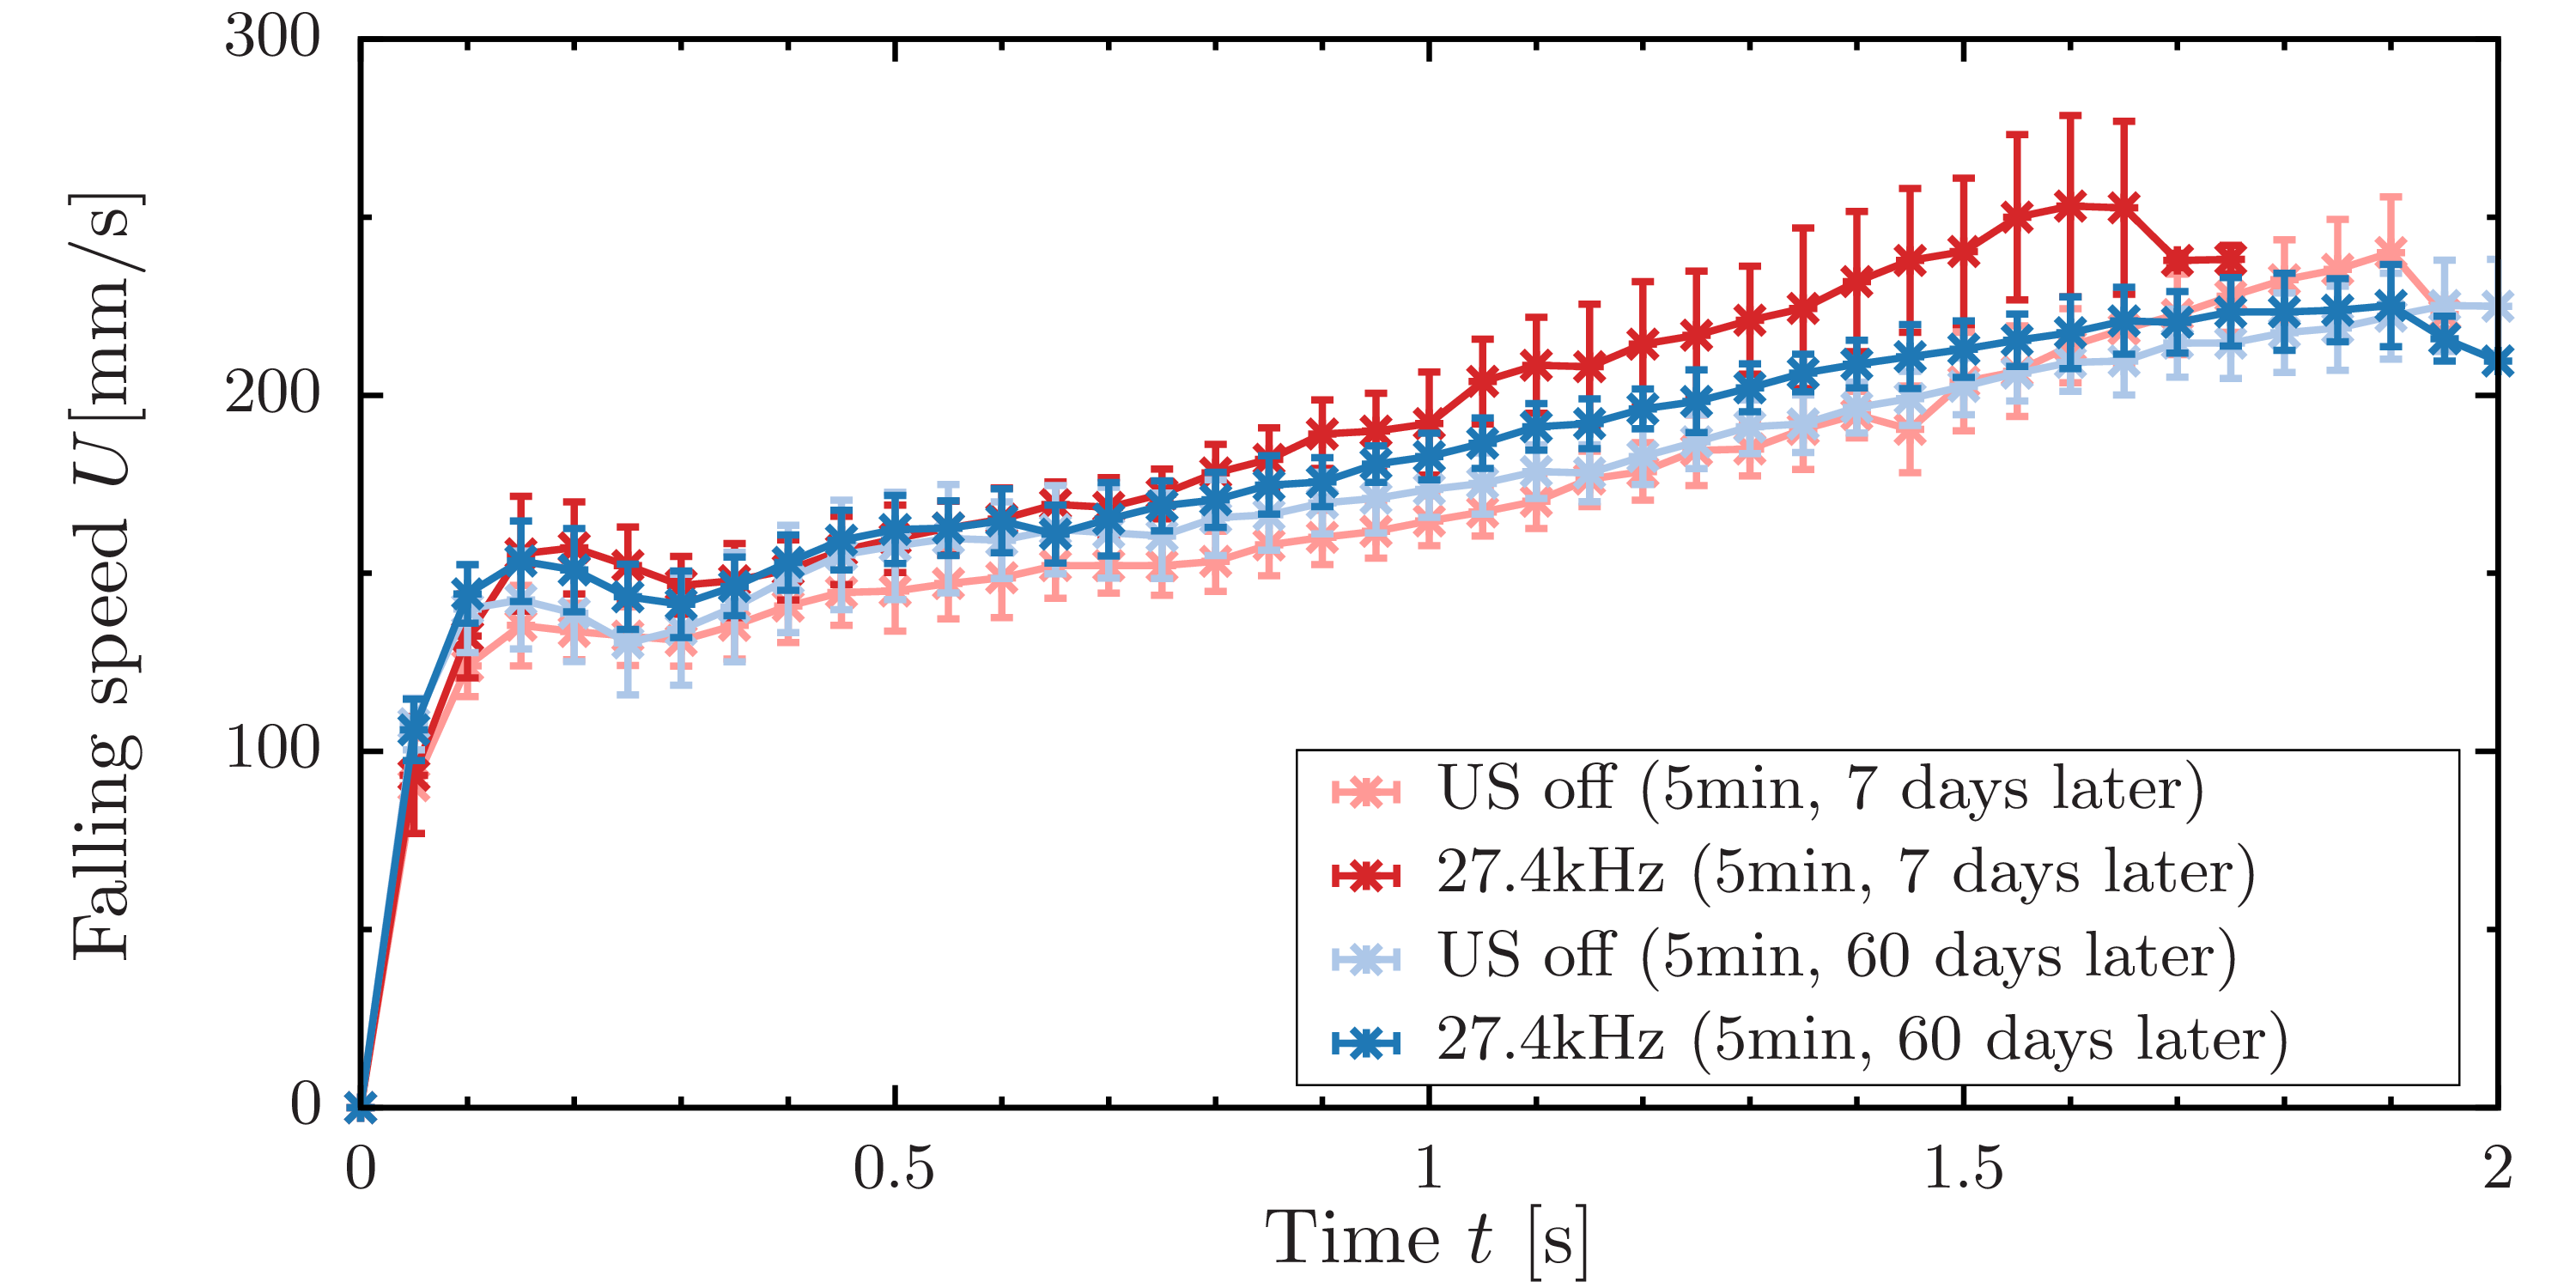
\includegraphics[width=11cm,clip]{X-Appendix/5.png}
    \caption{Falling velocity of a sphere in 1wt.\%PAA solution with and without ultrasound irradiationin tank B. Comparison of changes over time. (Interval 5 min.)}
    \label{fig:falling-5-2}
\end{figure}
\begin{figure}[H]
    \centering
    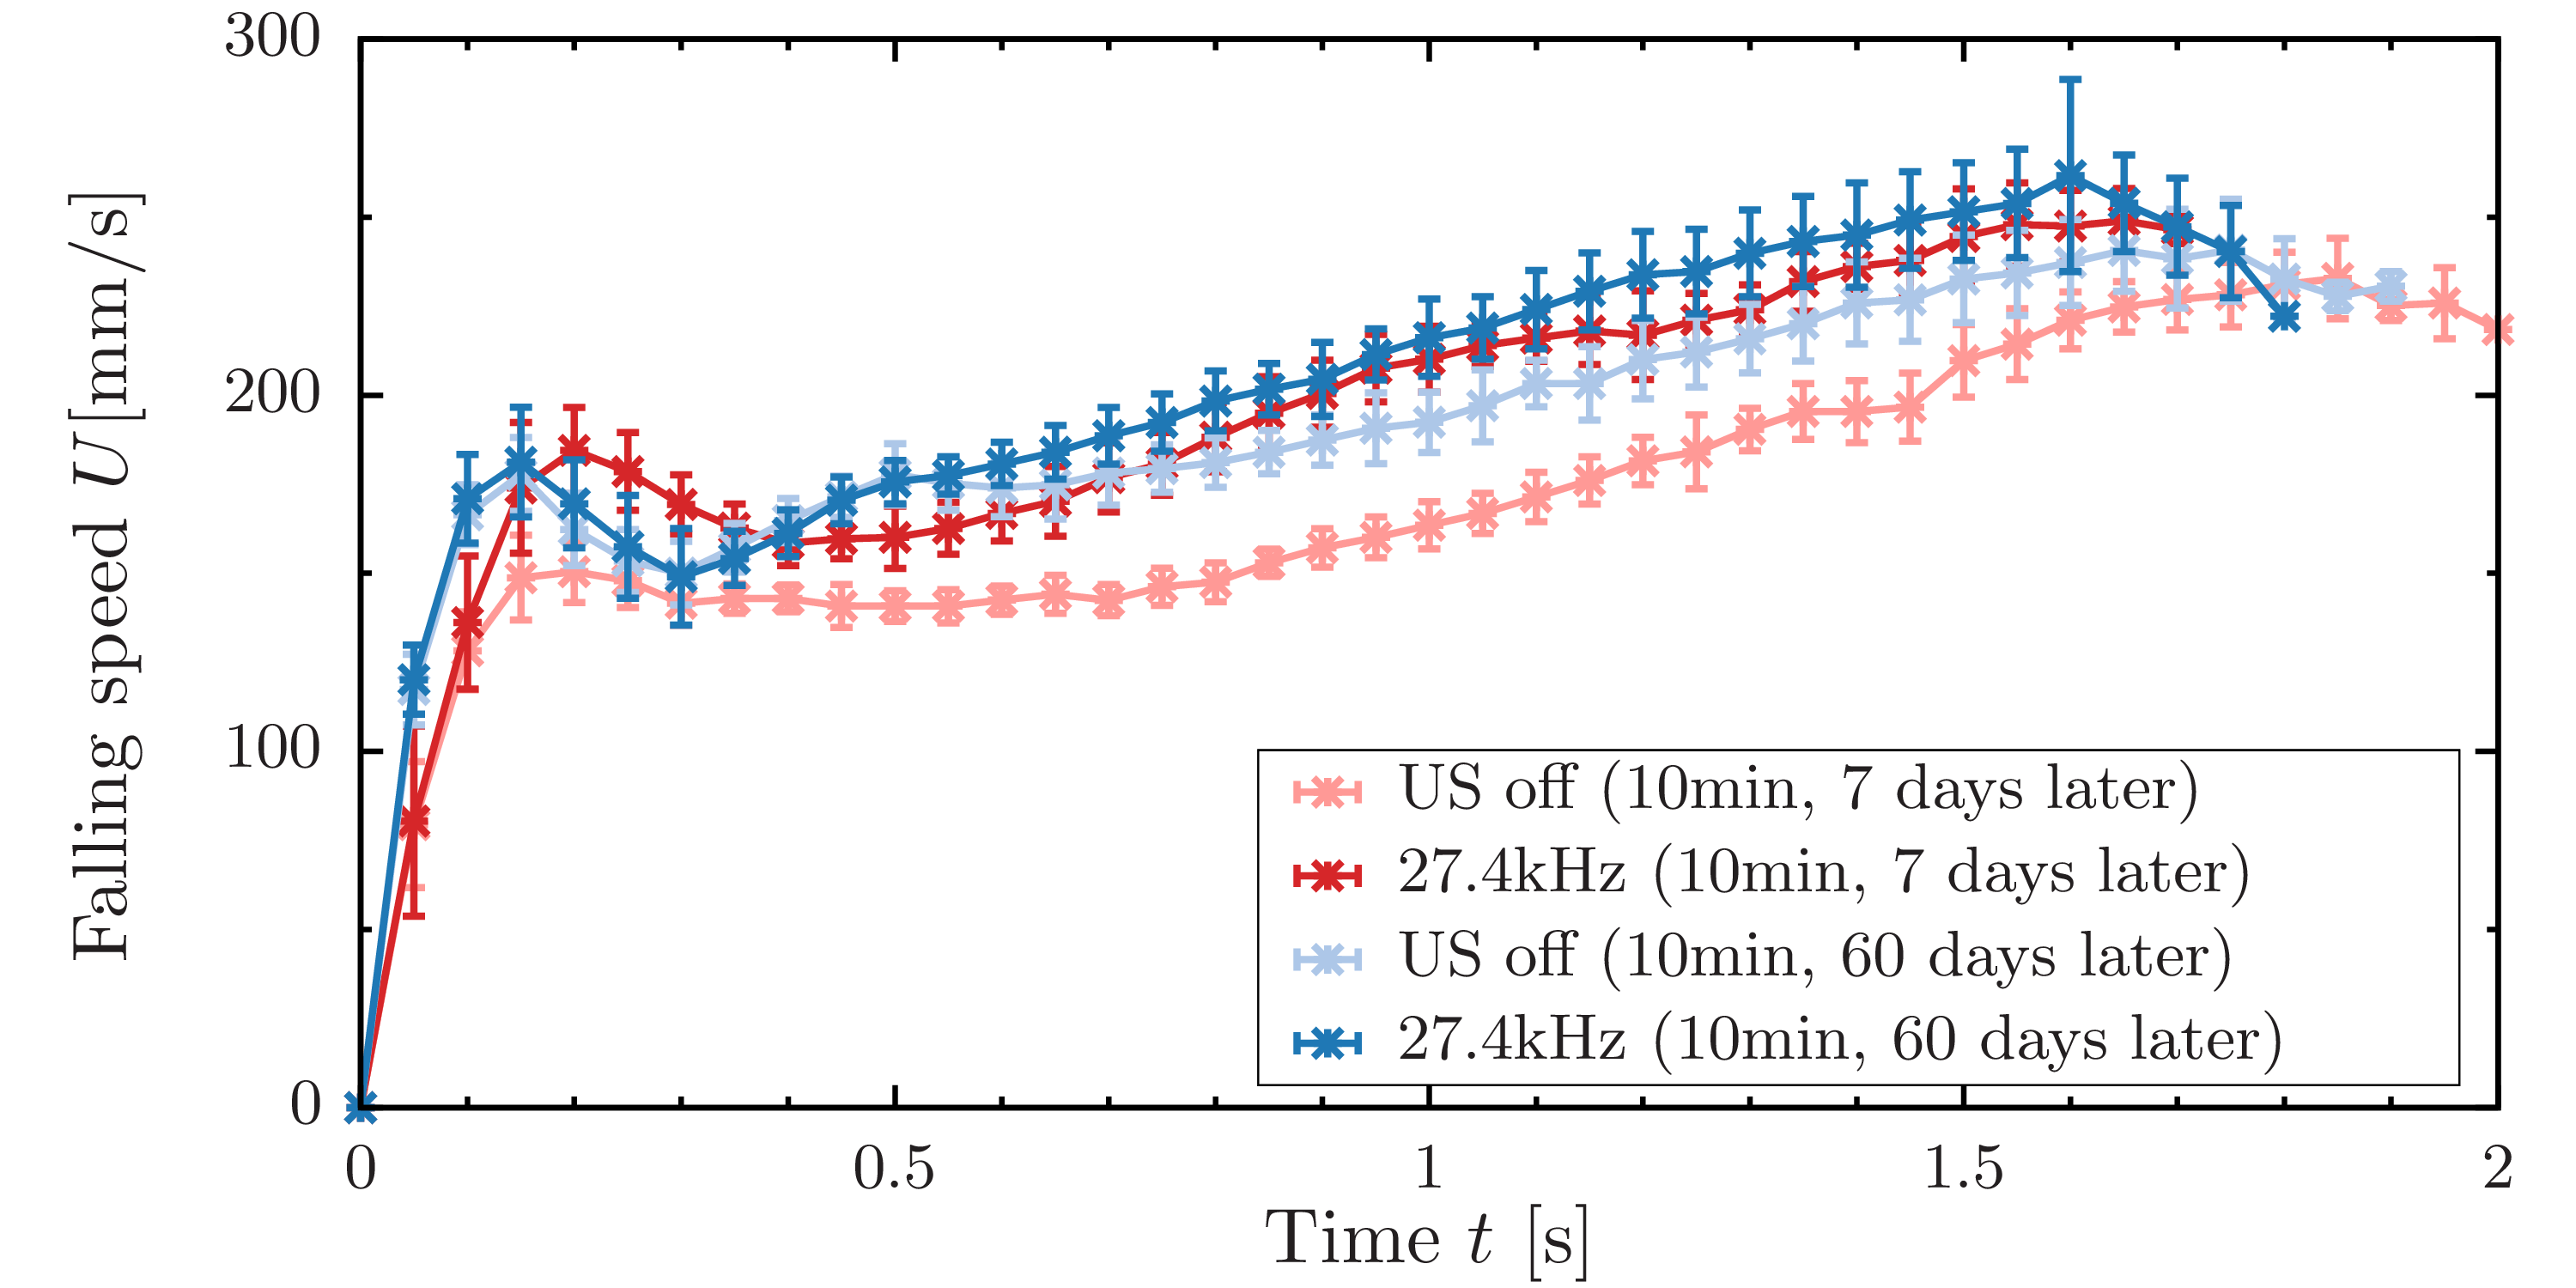
\includegraphics[width=11cm,clip]{X-Appendix/10.png}
    \caption{Falling velocity of a sphere in 1wt.\%PAA solution with and without ultrasound irradiationin tank B. Comparison of changes over time. (Interval 10 min.)}
    \label{fig:falling-10-2}
\end{figure}
\begin{figure}[H]
    \centering
    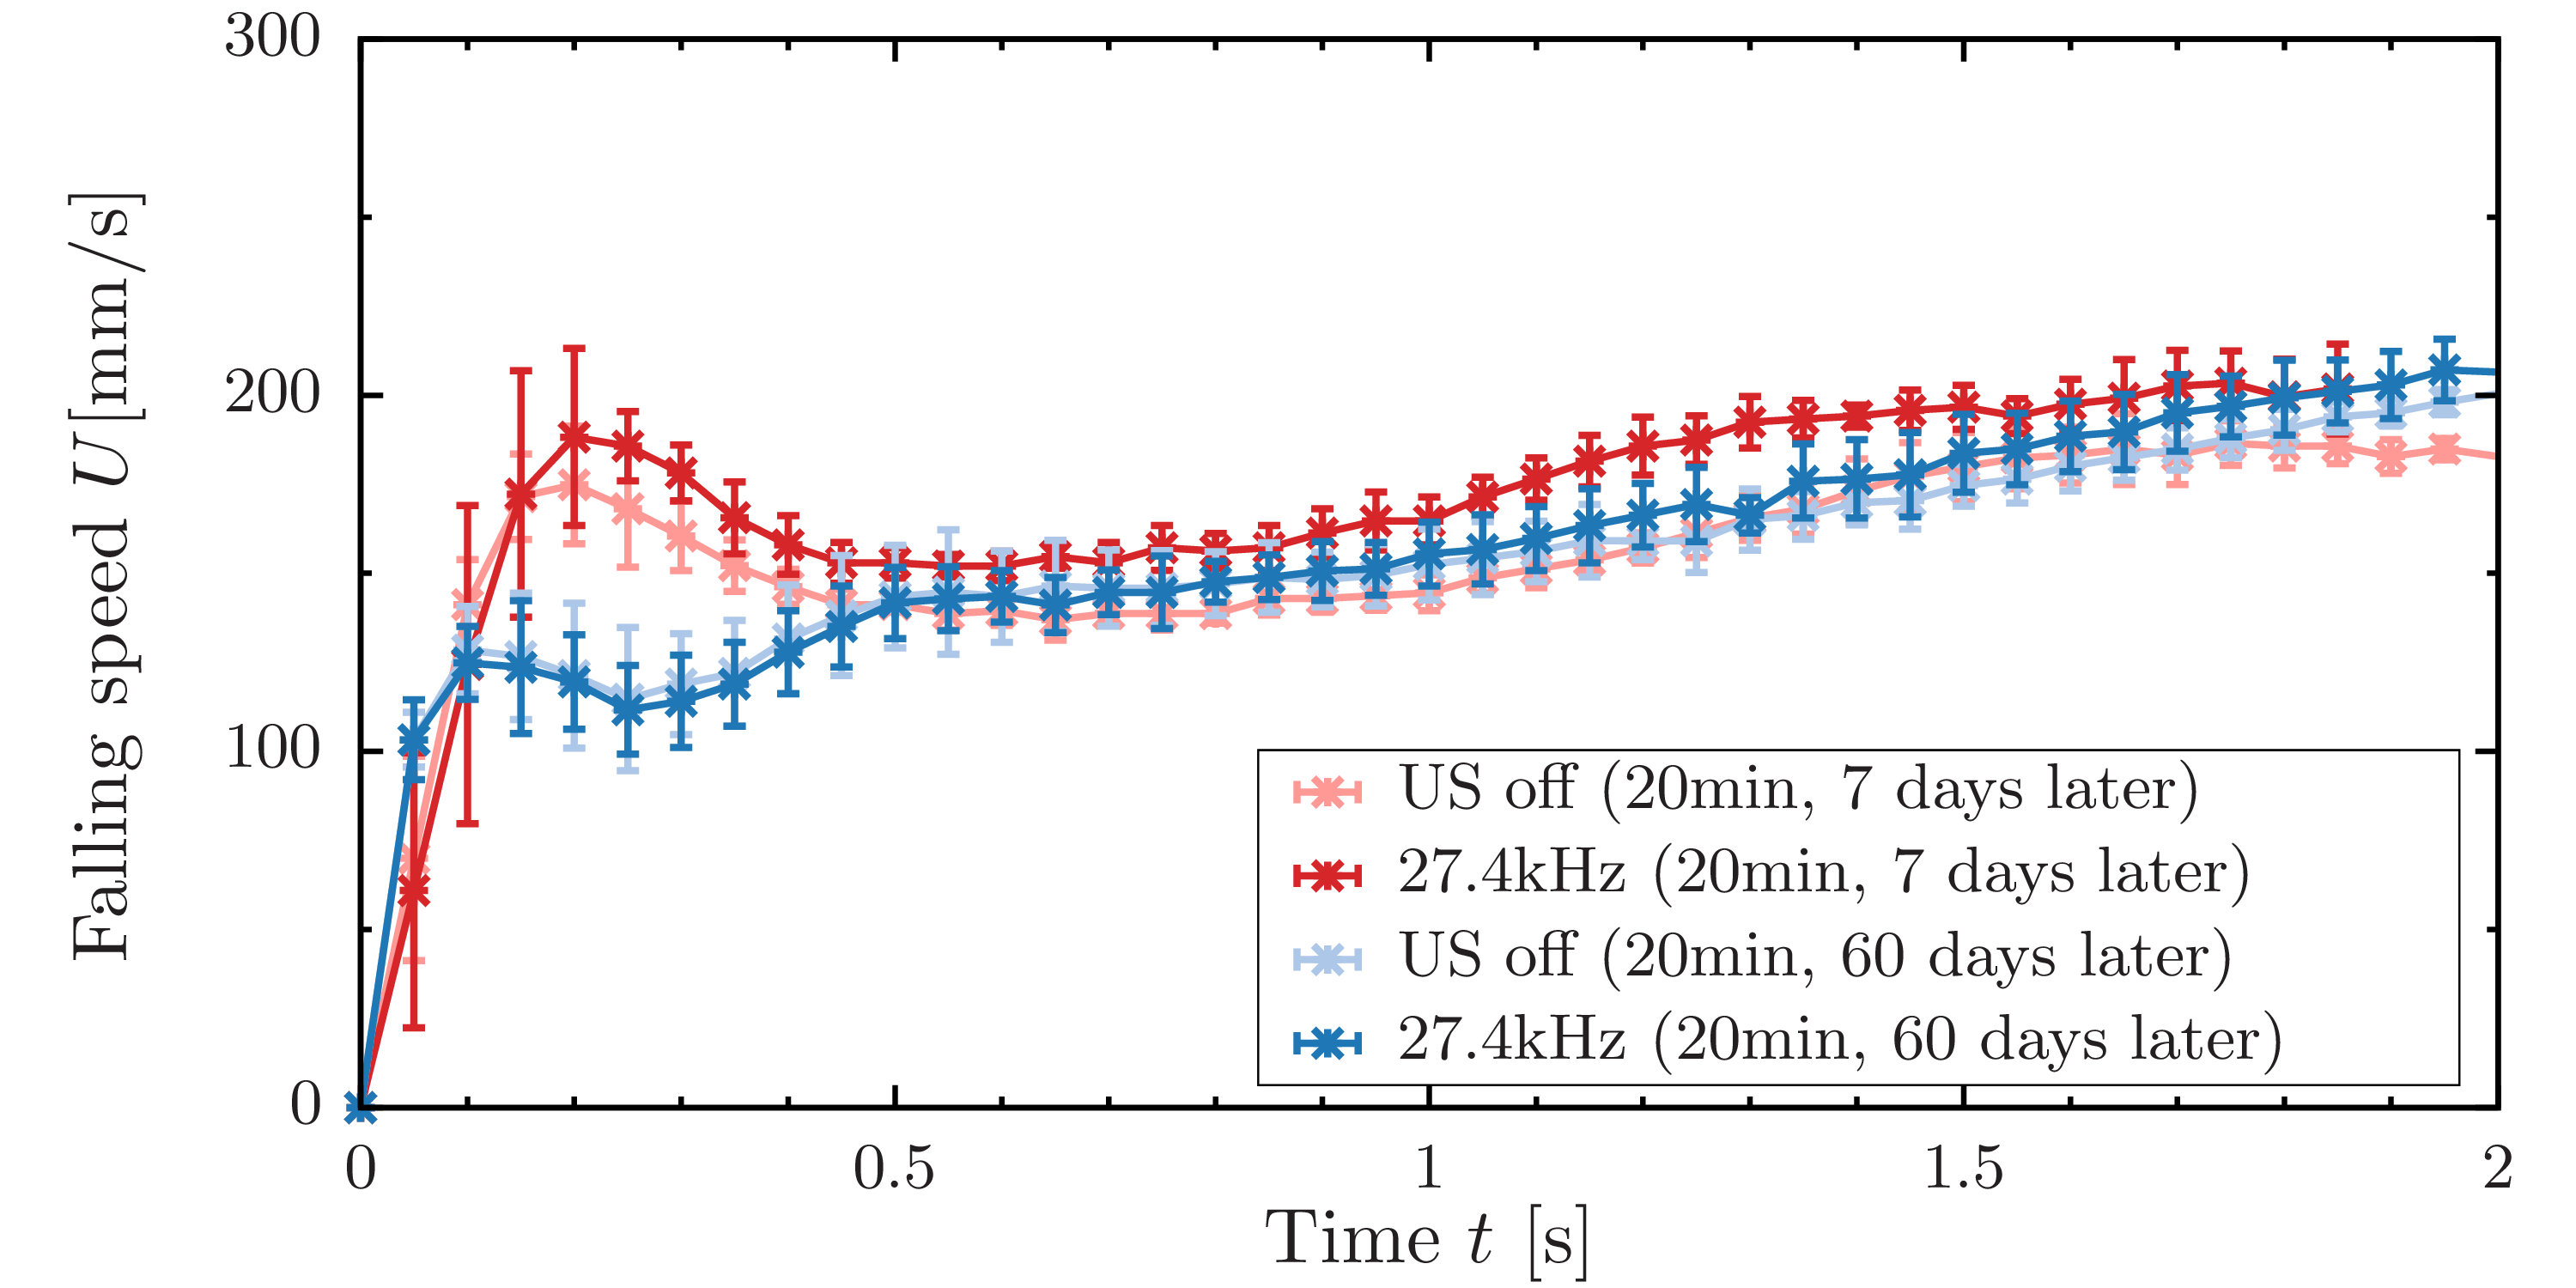
\includegraphics[width=11cm,clip]{X-Appendix/20.png}
    \caption{Falling velocity of a sphere in 1wt.\%PAA solution with and without ultrasound irradiationin tank B. Comparison of changes over time. (Interval 20 min.)}
    \label{fig:falling-20-2}
\end{figure}
